\documentclass[a4paper]{scrartcl}
\usepackage[
typ={ib},
fach=Informatik,
farbig
]{schule}


\usepackage{fontspec}
\usepackage{fourier-otf}
\usepackage{float}
\usetikzlibrary{arrows,calc,positioning}

\setmonofont[Scale = MatchLowercase]{jetbrainsmono-light}


\ifoot{% TODO: \usepackage{graphicx} required
	
	
\includegraphics[width=0.35\linewidth]{GHSE-Logo}
	
}

\usepackage[ngerman]{babel} 
\usepackage{tikz}
\usepackage{shellesc}
\usepackage{minted}
	\usepackage{url}
\usepackage{microtype}	
\usepackage[font=tiny,labelfont=bf]{caption}
\usepackage{xcolor}
\usepackage{color}
\usepackage{fancyvrb}
\date{}
\usetikzlibrary{positioning} 
\title{Java 24 Einstellungen}
\begin{document}
\maketitle



\section{Projekt erstellen}
Wähle bei der Erstellung eines neuen Projekts \texttt{Maven} als \texttt{Build sytem} und bei JDK irgendeine JDK mit Versionsnummer 24.

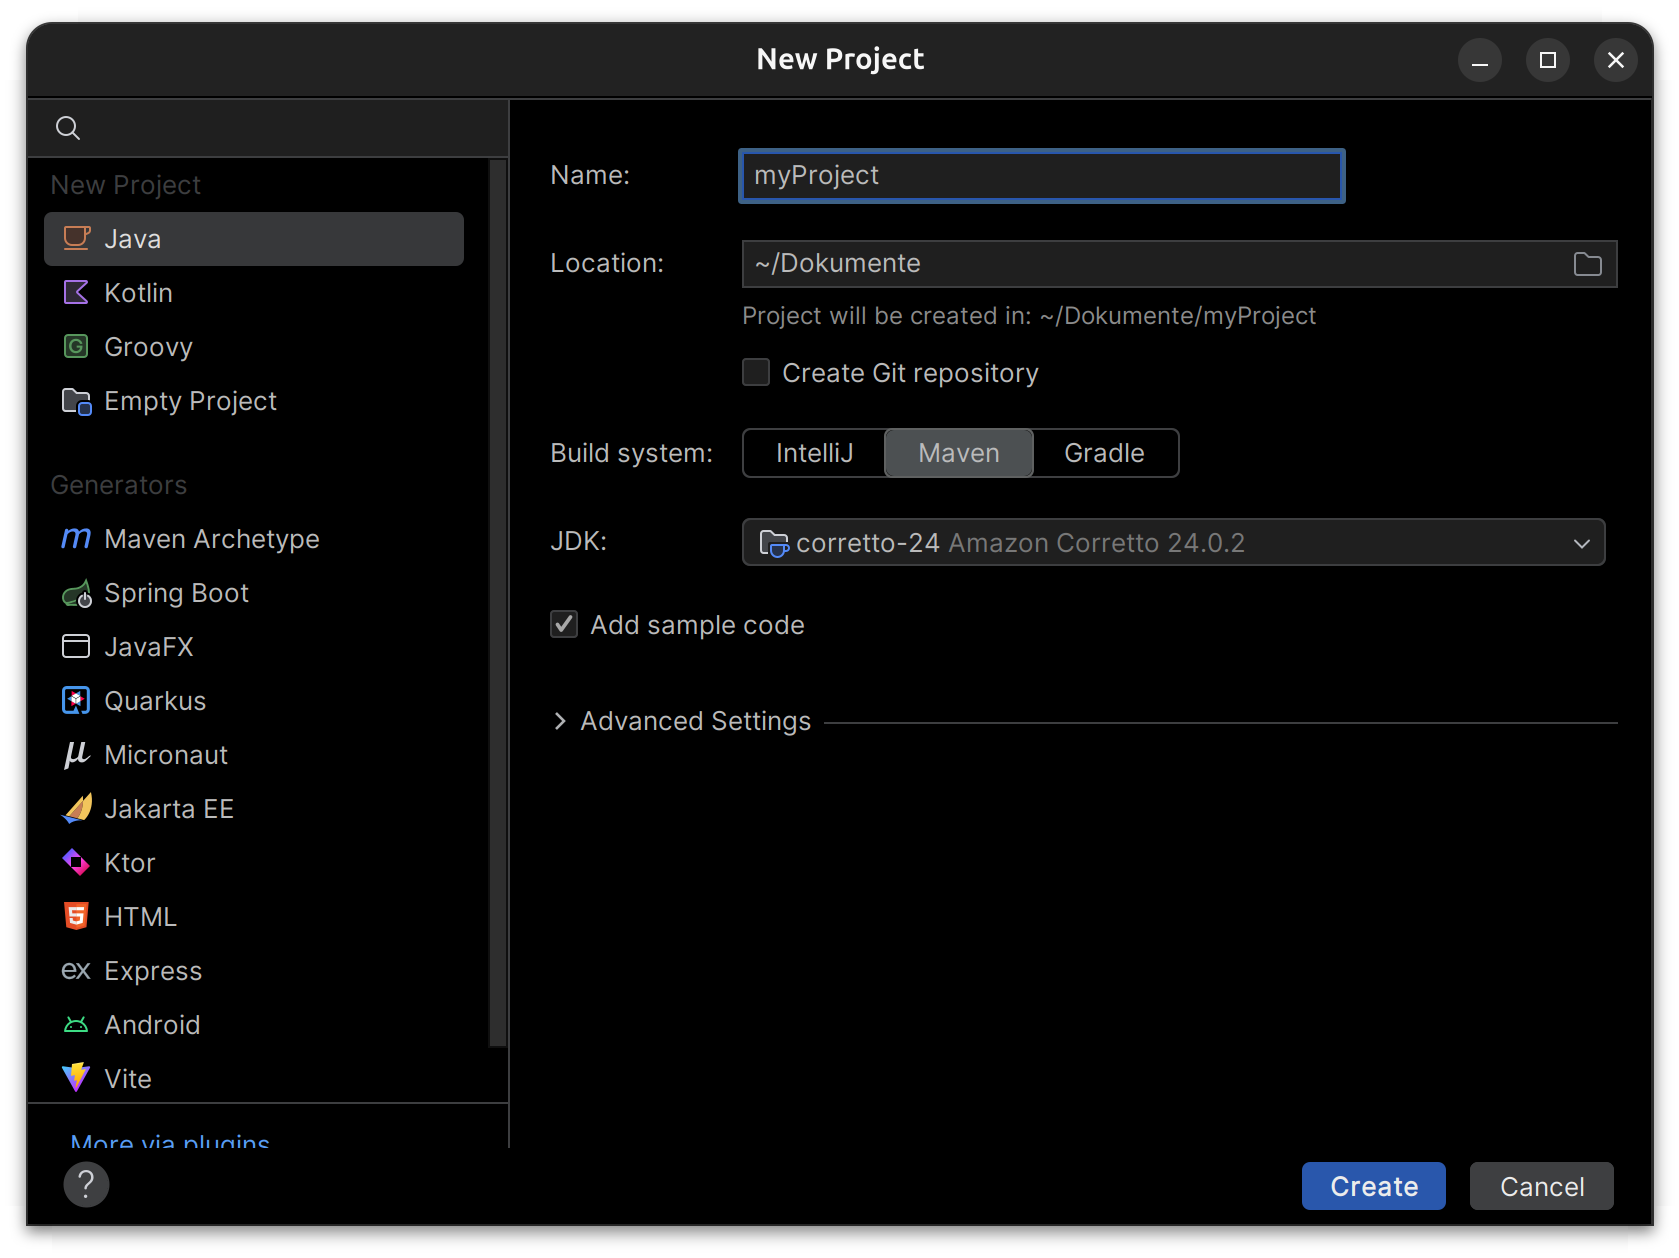
\includegraphics[width = \linewidth]{create}

\section{Projekteinstellungen ändern}
Wenn die Projekteinstellungen nicht mehr wie oben gesetzt sind, kannst du auf \texttt{File} und \texttt{Project Structure} klicken und die Einstellungen wieder korrigieren.

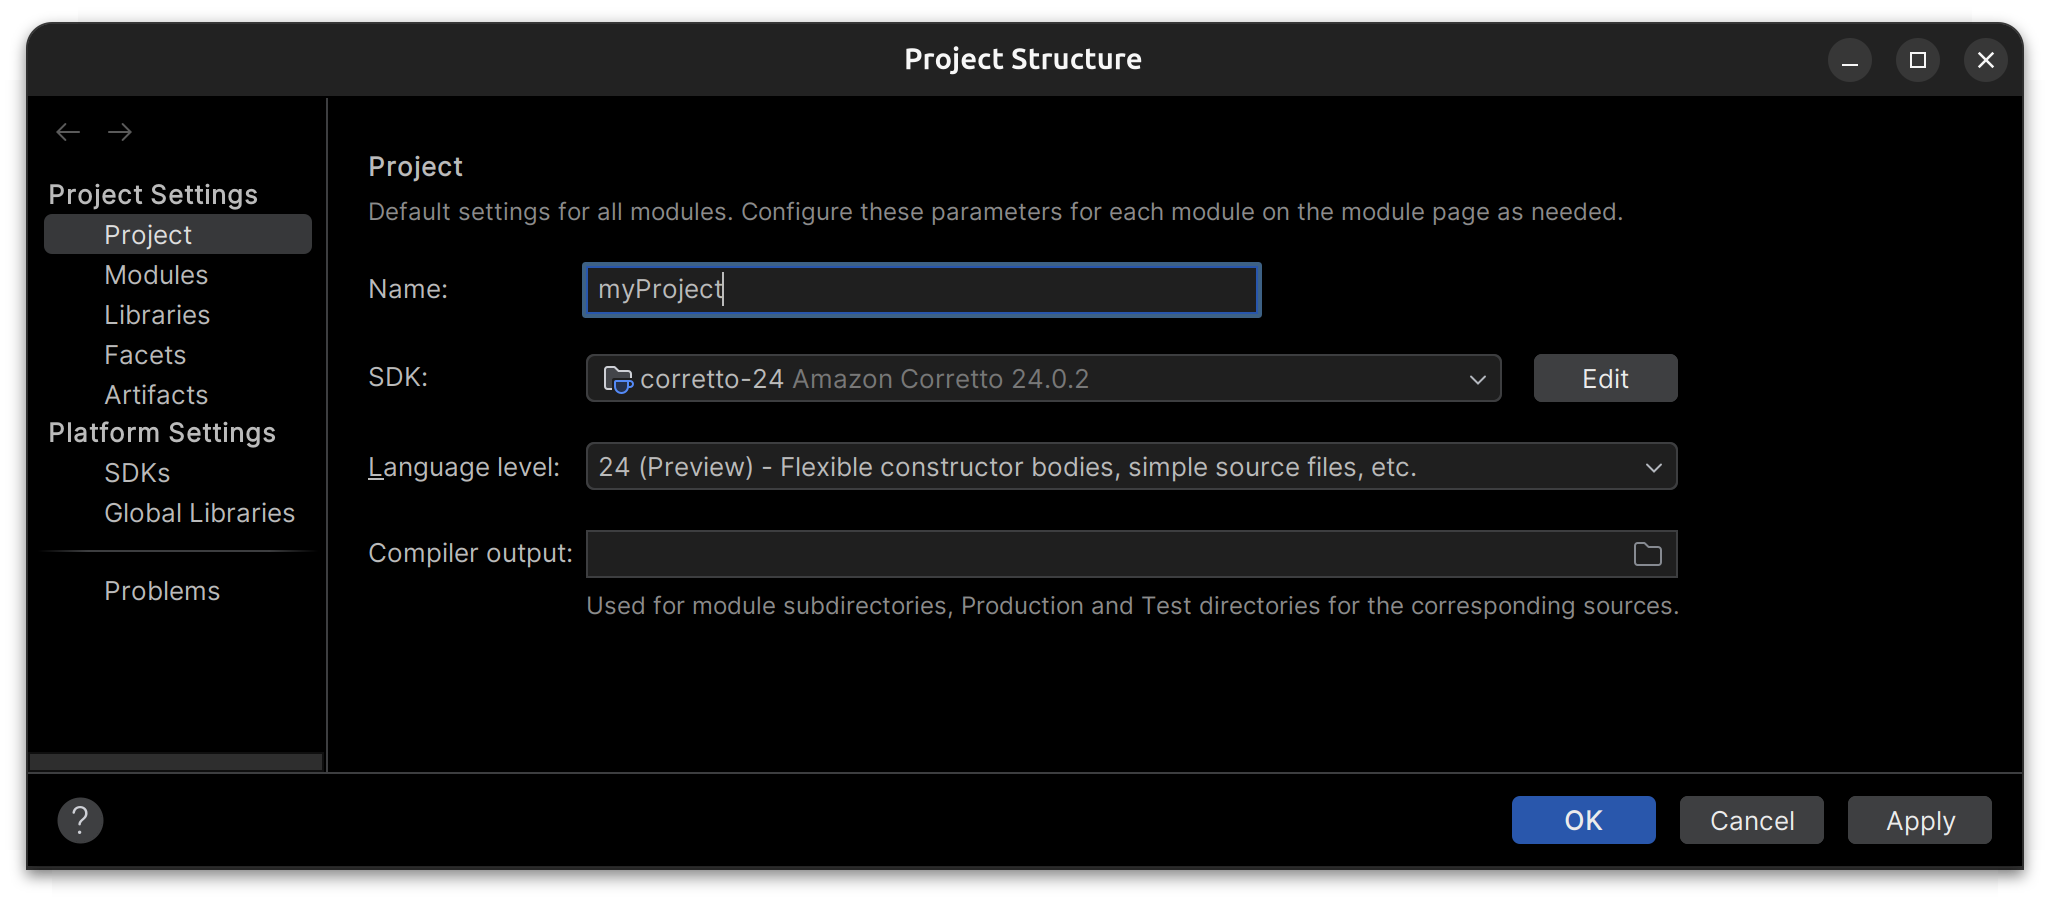
\includegraphics[width = \linewidth]{change}
\end{document}
